\documentclass[a4paper,11pt,oneside,titlepage,openany,onecolumn]{scrreprt}

%%%%%%%%%%%%%%%%%%%%%%%%%%%%%%%%%%%%%%%%%%%%%%%%%%%%%%%%%%%%%%%%%%%%%%%%%%%%%%%%%%%%%%

% General settings (input encoding, font encoding, font, language)
% ****************************************************************************************
\usepackage[utf8]{inputenc} % character encoding used in input file
\usepackage[T1]{fontenc} % specifies the encoding used in the fonts
\usepackage{lmodern} % provides more support for non-ASCII characters than cm-super
\usepackage{microtype} % improves line-filling when using PDFLaTeX
\usepackage[ngerman,english]{babel} % last language is considered the main one
%\usepackage{helvet}
\renewcommand{\familydefault}{\sfdefault} % select a sans serif font family
%
% ****************************************************************************************

% ****************************************************************************************
% Basic packages (graphics, tables, code highlighting, epigraphs)
% ****************************************************************************************
\usepackage{graphicx} % provides enhanced support for including graphics and images
% \usepackage{epstopdf}
\graphicspath{{img/}} % list of directories in which to search for graphics files 
\usepackage[table]{xcolor} % extends the color capabilities of LaTeX
\usepackage{color}
\definecolor{MSBlue}{rgb}{.204,.353,.541} 
\definecolor{trueblue}{rgb}{0.0, 0.45, 0.81}
\definecolor{onyx}{rgb}{0.06, 0.06, 0.06}
\definecolor{mygruen}{rgb}{0.4660, 0.6740, 0.1880}
\definecolor{plotblue}{rgb}{0, 0.4470, 0.7410}
\definecolor{myrot}{rgb}{0.8500, 0.3250, 0.0980}
\definecolor{mygreen}{RGB}{28,172,0} % Matlab comment
\definecolor{mylilas}{RGB}{170,55,241} % Matlab String
\definecolor{MCIBLUE}{RGB}{0,73,131}
\usepackage{tabularx} % extends functionality of the traditional tabular environment
\usepackage{array}
\usepackage{booktabs}
\usepackage{dcolumn}
\usepackage{multirow}

\usepackage{grffile} % improves support for file names with multiple dots
\usepackage{minted} % used to format and highlight programming language source code
% \usepackage{tocloft} % provides means of controlling the typographic design of the ToC
\KOMAoptions{toc=flat} % Glatte Abstände
\KOMAoptions{toc=indent} % Eingerückte Ebenen im Inhaltsverzeichnis
\setlength{\marginparwidth}{2cm}
\usepackage{todonotes}
\usepackage{pst-all} %% erweiterte Zeichenbefehle

% ****************************************************************************************
% Drawing and plotting
% ****************************************************************************************
\usepackage{pgfplots} % provides a high-level interface for creating plots and charts
\pgfplotsset{compat=newest} % sets the compatibility level to the newest version
\usetikzlibrary{plotmarks} % provides various markers (symbols) that can be used
\usetikzlibrary{arrows.meta} % allows customization of arrow tips for paths and arrows
\usepgfplotslibrary{patchplots} % provides additional functionality for handling patches
\usepgfplotslibrary{external} % provides functionality for externalizing plots
\tikzexternalize % activates the externalization feature for TikZ
\newlength\figureheight % declares a new length used to store used to store dimensions
\newlength\figurewidth % declares a new length used to store used to store dimensions
\usepackage{circuitikz} % used for drawing electrical circuits
\usepackage{tikz}
\usepackage{tikzscale}

% ****************************************************************************************
% Mathematics and physics
% ****************************************************************************************
\usepackage{amsmath,amssymb,amsfonts,amstext}
\usepackage{mathtools}
\usepackage{mathrsfs}

%% -> SI-Einheiten
\usepackage{siunitx}
% Einstellungen für SI-Einheiten
\sisetup{
	locale = DE,                        % Deutsche Einstellungen
	output-decimal-marker = {,},        % Dezimaltrennzeichen auf "," setzen
	exponent-product = \cdot,           % Exponenten mit "·" trennen
	per-mode = symbol-or-fraction,      % "pro" als Symbol oder Potenz
	parse-numbers = true,               % Automatische Nummerninterpretation
	bracket-numbers = false             % Entfernt Klammern bei negativen Exponenten
}

% ****************************************************************************************
% Referencing and citing
% ****************************************************************************************
\usepackage[
	format=plain,% typeset caption as normal paragraph
	labelformat=simple,% typeset label as name and number
	labelsep=period,% caption label and text separated by period and space
	textformat=simple,% caption text typeset as is (without additional formatting)
	justification=justified,% sets the justification of the caption text to be justified
	singlelinecheck=true,% automatically center short captions
	font=small,% set font size to small
	labelfont=bf,% set bold font for label
	width=.75\textwidth% set fixed width for caption
]{caption} % customize the formatting of captions
\usepackage{subcaption}
\captionsetup[figure]{
	labelfont=bf,                   % Beschriftung für Abbildungen fett
	textfont=normal,                % Text normal
	labelsep=space,                 % Punkt nach der Beschriftung
	%belowskip=10pt
}
\captionsetup[table]{
	labelfont=bf,                   % Beschriftung für Tabellen fett
	textfont=normal,                % Text normal
	labelsep=space,                 % Punkt nach der Beschriftung
	belowskip=10pt
}
% Titel von Abbildungen und Tabellen ändern
\renewcommand\figurename{Abbildung}
\renewcommand\tablename{Tabelle}
% ****************************************************************************************

% \usepackage{hyperref} % hypertext marks (should be loaded last but before geometry)
% \hypersetup{
%     colorlinks,% colours the text of links and anchors (instead of borders)
% 	linkcolor={MCIBLUE},%
% 	citecolor={MCIBLUE},%
% 	urlcolor={MCIBLUE},%
%   % pdftitle={\thesisTitle},% PDF display and information options
% 	% pdfsubject={\thesisType},%
% 	% pdfauthor={\thesisStudent},%
% 	pdfkeywords={thesis},%
% 	pdfcreator={pdflatex},%
% 	pdfproducer={LaTeX with hyperref}%
% }
\usepackage[
bookmarks=true,
bookmarksopen=true,
bookmarksnumbered=true,
pdfborder={0 0 0},
colorlinks=true,
linkcolor=MCIBLUE,
citecolor=MCIBLUE,
urlcolor=MCIBLUE
]{hyperref}
\usepackage[capitalise]{cleveref} % enhances cross-referencing features
\crefformat{equation}{(#2#1#3)}
\Crefformat{equation}{Equation~(#2#1#3)}
\crefname{figure}{Abbildung}{Abbildungen} % Singular und Plural für Abbildungen
\crefname{table}{Tabelle}{Tabellen}       % Singular und Plural für Tabellen
\crefname{equation}{Gleichung}{Gleichungen} % Singular und Plural für Gleichungen

% \Crefname{figure}{Abbildung}{Abbildungen} % Für den Satzbeginn mit großem Anfangsbuchstaben
% \Crefname{table}{Tabelle}{Tabellen}
% \Crefname{equation}{Gleichung}{Gleichungen}
% ****************************************************************************************

% ****************************************************************************************
% Bibliography settings
% ****************************************************************************************
% IEEEtran BibTeX style downloaded from: https://www.ctan.org/pkg/ieeetran
\bibliographystyle{IEEEtran} % choose the reference style
%
% ****************************************************************************************
% Glossary (acronyms, list of symbols) settings
% ****************************************************************************************
\usepackage[acronym,nomain,nonumberlist,nopostdot,sort=def,toc]{glossaries}
\renewcommand*{\glstextformat}[1]{\textcolor{black}{#1}} % make links appear black
\newglossary[slg]{symbolslist}{syi}{syg}{List of Symbols} % define custom glossary
\glsaddkey% define custom key
	{unit}% key
	{\glsentrytext{\glslabel}}% default value
	{\glsentryunit}% command analogous to \glsentrytext
	{\GLsentryunit}% command analogous to \Glsentrytext
	{\glsunit}% command analogous to \glstext
	{\Glsunit}% command analogous to \Glstext
	{\GLSunit}% command analogous to \GLStext
\glssetnoexpandfield{unit}
\makeglossaries % create makeindex files
% glossary of symbols is formatted as a longtable with three columns
\newglossarystyle{symbolsliststyle}{%
	\setglossarystyle{long3col}% style based on long3col
	\renewenvironment{theglossary}{%
		\begin{longtable}{lp{\glsdescwidth}>{\arraybackslash}p{2cm}}}%
		{\end{longtable}}%
	\renewcommand*{\glossaryheader}{% change the table header
		\bfseries Symbol & \bfseries Beschreibung & \bfseries Einheit\\\midrule%
		\endhead%
	}%
	\renewcommand*{\glossentry}[2]{% change the displayed items
		\glstarget{##1}{\glossentryname{##1}}% name
		& \glossentrydesc{##1}% description
		& $\glsentryunit{##1}$% unit
		\tabularnewline%
	}%
}


% ****************************************************************************************
% Page layout and headers
% ****************************************************************************************
\usepackage[
    includeheadfoot,% includes the head of the page into total body
	ignoremp,% disregards marginal notes in determining the horizontal margins
	nomarginpar,% shrinks spaces for marginal notes to 0pt
	hmargin=1.25in,% left and right margin
	vmargin=1in,% top and bottom margin
	headheight=14pt%  height of header
]{geometry} % specify page layout (paper name and orientation specified in doc class)
%\usepackage{parskip} % helps in implementing paragraph layouts
\KOMAoptions{parskip=half} % parskip=off, % parskip=half

\usepackage{fancyhdr} % header and footer settings
\pagestyle{fancy} % set page style to 'fancy'
\renewcommand{\chaptermark}[1]{\markboth{\thechapter.\ #1}{}}
\fancyhf{} % clear all header and footer fields
\fancyhead[L]{\nouppercase\leftmark} % set left header location (chapter)
\fancyfoot[C]{\thepage} % set center footer location (page count)


% ****************************************************************************************
% Matlab Code
% ****************************************************************************************
\usepackage{listings}
% MATLAB Code
\lstset
{language=Matlab,%
	basicstyle=\footnotesize,
	breaklines=true,%
	captionpos=b,
	frame = single,
	morekeywords={matlab2tikz},
	keywordstyle=\color{blue},%
	morekeywords=[2]{1}, keywordstyle=[2]{\color{black}},
	identifierstyle=\color{black},%
	stringstyle=\color{mylilas},
	commentstyle=\color{mygreen},%
	showstringspaces=false,%
	%numbers=left,%
	%numberstyle={\footnotesize \color{black}},%
	%stepnumber=5, %
	%numbersep=9pt, % 
	emph=[1]{for,end,break},emphstyle=[1]\color{red}, %
	emph=[2]{all}, emphstyle=[2]\color{mylilas},    
}

% ****************************************************************************************

\usepackage{lipsum}

% %% -> Layout Überprüfung
% \usepackage{layout}
% \usepackage{xspace}

% %% -> Einrücken von und Abstand zwischen Absätzen
% \setlength{\parindent}{0em}
% \setlength{\parskip}{1.5ex plus0.5ex minus0.5ex}

% %% -> Tabulator Funktion
% \newcommand\tab[1][1cm]{\hspace*{#1}}

% %% -> Weniger Warnungen wegen überfüllter Boxen
% \tolerance = 9999
% \sloppy



%% --------------------------------------------------------------------- %%

%% -> Bildnummerierung ist logisch mit Kapitelnummerierung
% \numberwithin{figure}{chapter}
% \numberwithin{table}{chapter}
% \numberwithin{equation}{chapter}
%\numberwithin{equation}{subsection}
%% --------------------------------------------------------------------- %%



%% --------------------------------------------------------------------- %%

%% -> Für das Symbolverzeichnis
% \usepackage[toc, hyperfirst = false, acronym, nonumberlist]{glossaries}
% \makeglossaries
%\input{Symbols_Acronym/symbols}
%\input{Symbols_Acronym/acronym}
%% --------------------------------------------------------------------- %%

% Boolesche Variable f"ur Bachelor-/Masterarbeit oder Bericht
\newboolean{thesis}
\loadglsentries{tex/defsymbols.tex}

% Titlepage

\def\title{Titel der Arbeit}
\def\study{Mechatronics \& Smart Technologies}
\def\thesis{Masterarbeit}
\def\degree{"Master of Science in Engineering"}
\def\student{Max Mustermann}
\def\matnr{666}
\def\address{A-PLZ Ort, Stra{\ss}e Hausnummer}
\def\reviewerone{Dr. Martina Musterfrau}
\def\reviewertwo{Dr. Markus Mustermann}

%%%%%%%%%%%%%%%%%%%%%%%%%%%%%%%%%%%%%%%%%%%%%%%%%%%%%%%%%%%%%%%%%%%%%%%%%%%%%%%%%%%%%%
\begin{document}
    \selectlanguage{ngerman}
    \pagenumbering{alph} % use lowercase letters for page numbering
    % ****************************************************************************************
\thispagestyle{empty} % suppress the headers and footers on the current page
\pdfbookmark[0]{Title page}{titlepage} % sets a PDF bookmark
\thispdfpagelabel{} % set page number shown in the tool bar of a PDF viewer
\begin{center}
\sffamily
%\put(-30,-685){\includegraphics[width=1.15\linewidth]{BG}}
\textbf{\huge\title}

\vspace*{3cm}

\framebox[13cm]{\textbf{\huge\thesis}}

\vspace*{1.5cm}
\Large zur Erlangung des akademischen Grades

\vspace*{1cm}

\Large \degree

\vspace*{1.5cm}

\Large Studiengang:

\textbf{\Large\study}

\Large Management Center Innsbruck

\vspace*{1.5cm}

Betreuende/r:

\textbf{\Large\reviewerone}

%\vspace*{2cm}

Begutachtende/r:

\textbf{\Large\reviewertwo}

\vspace*{1cm}

Verfasser/-in:

\textbf{\Large\student}

\textbf{\Large\matnr}
\end{center}

\newpage
 % include title page
    \pagenumbering{Roman}  % use uppercase roman numerals for page numbering
    \thispagestyle{plain} % format page style for current page
\pdfbookmark[0]{Eidesstattliche Erklärung}{Eidesstattliche Erklärung} % sets a PDF bookmark


\chapter*{Eidesstattliche Erklärung}
\glqq Ich erkläre hiermit an Eides statt, dass ich die vorliegende Arbeit selbstständig angefertigt habe. Die aus fremden Quellen direkt oder indirekt übernommenen Gedanken sind als solche kenntlich gemacht. Die Arbeit wurde bisher weder in gleicher noch in ähnlicher Form einer anderen Prüfungsbehörde vorgelegt und auch noch nicht veröffentlicht.\grqq\\[5\baselineskip]
\vspace{2cm}
\begin{tabularx}{\textwidth}{@{}p{5cm}Xp{5cm}@{}} % @{} eliminates default padding
    \hrulefill & & \hrulefill \\
    Ort, Datum & & Unterschrift
\end{tabularx}
% % include eid
    \selectlanguage{ngerman}
\section*{\centering Kurzfassung}
Text Text Text Text Text Text Text Text Text Text Text Text Text Text Text Text Text Text Text Text Text Text Text Text ...

% Bitte 3-5 deutsche Schlagw"orter eingeben, die die Arbeit charakterisieren:
\paragraph*{Schlagw"orter:} Schlagwort 1, Schlagwort 2, Schlagwort 3, Schlagwort 4, Schlagwort 5
\newpage
 % include abstract (german version)
    \thispagestyle{plain} % format page style for current page
\selectlanguage{english} % switch language to English
\pdfbookmark[0]{\abstractname}{abstractenglish} % sets a PDF bookmark
\chapter*{\abstractname}
Text Text Text Text Text Text Text Text Text ...

\textbf{\textit{Keywords}} --- artificial intelligence, machine learning, cybersecurity

\selectlanguage{ngerman} % switch language to German % include abstract (english version)
    \pdfbookmark[0]{\contentsname}{toc} % sets a PDF bookmark
    \tableofcontents
    \newcounter{romanpagecount} % create a new counter
    \setcounter{romanpagecount}{\value{page}} % capture the current page number
    \clearpage
    \pagenumbering{arabic} % use Arabic numerals for page numbering
	% --> add content of thesis here
    \chapter[Introduction]{Introduction}

\section{Motivation and Problem Statement}

%globale Demenzstatistiken (Alzheimer Int., WHO)
\cite{alzint_dementia_statistics}, \cite{who_dementia_factsheet}

%Bedarf an nicht-pharmakologischen Ansätzen
\cite{Zucchella.2018}

%Frühstudien zur 40-Hz-Stimulati (z.B. Gamma-Wellen, Reduktion von Amyloid in Mäusen)
\cite{Mably.2018}, \cite{Iaccarino.2016}, \cite{Martorell.2019}

\section{Objectives of the Thesis}

Erl"autern Sie an dieser Stelle \emph{genau} was ihre Aufgabe ist. Gegebenfalls grenzen Sie auch die Teile aus, welche nicht im Umfang der Arbeit liegen. Dies kann Ihnen gegen Ende ihrer Arbeit bei der Argumentation helfen.

\section{Structure of the Thesis}

Geben Sie in diesem Abschnitt eine grobe Vorausschau auf den Aufbau der Arbeit. Die Arbeit k"onnte empirisch motiviert sein und mit der Auswertung eines Experimentes beginnen oder theoreitsch und somit logischerweise mit einem Theoriekapitel beginnen.


Etst
    \chapter[Formatierungen]{Formatierungen von "Uberschriften und Text in Latex}

In Latex brauchen Sie sich um Formatierungen im Prinzip nicht k"ummern. Es ist lediglich notwendig, dass Sie Kapitel, Abschnitte, Unterabschnitte und so weiter als solche deklarieren.

Multiple Leerzeichen        werden von Latex einfach gel"oscht. Haben Sie einen Absatz beendet (nach 3 bis 4 S"atzen), dann lassen Sie durch ein zweimaliges ''Enter'' eine Zeile Abstand. Der Absatz wird je nach globaler Einstellung einger"uckt oder abgesetzt.

Wollen Sie im Text etwas hervorheben, dann verwenden Sie \emph{hervorgehoben}. Die Hervorhebung wird von Latex automatisch dem jeweiligen Textstil angepasst. Sie k"onnen aber auch etwas explizit \textbf{fett}, \textit{kursiv} oder \underline{unterstrichen} setzen, wobei dies mit Vorsicht zu genie"sen ist.

\section[Abschnitt]{Das wäre ein Abschnitt}

Mit etwas Text ...

\subsection[Unterabschnitt]{Bzw. ein Unterabschnitt}

Wie Ihnen vielleicht schon aufgefallen ist, vergr"o"sert \LaTeX nach einem ''.'' den Abstand geb"uhrlich f"ur ein Satzende. Falls dies nicht ben"otigt wird z.B.~hier, sollte dies h"andisch verhindert werden.

\paragraph{Gliederungsebene 3} Die n"achste Gliederungsebene wird nicht mehr nummeriert.

\LaTeX kennt auch Aufz"ahlungen wobei es diese mit
\begin{enumerate}
\item Nummerierung
\item\label{enum-ebene} auf der ersten Ebene
\item oder
\begin{itemize}
\item ohne Nummerierung
\item auf der 2.~Ebene gibt.
\end{itemize}
\end{enumerate}
Es gibt eine ganze Reihe von weiteren Formatierungsm"oglichkeiten. Z.B.~behandelt {\LaTeX} die erste Seite eines Kapitels anders als alle folgenden. Dies f"allt insbesondere bei der Seitenzahl und der Kopfzeile auf.

    \chapter{Analysis of the Current VCA-Based System}

\section{Overview of the Current VCA System}
This section provides an overview of the existing Voice Coil Actuator (VCA)-based setup. The System consists of seven main parts. 

\begin{itemize}
    \item Spring frame (Minimizing the loss of vertical motion transmitted to the node)
    \item Magnet Housing (fixed Magnetic field is always formed)
    \item Bobbin Coil (Magnetic field is formed only when current flows)
    \item Node (Transmitting vertical motion directly to the human body as sound and vibration)
    \item Node screw (fixes the node to the bobbin coil)
    \item Rubber frame (Suppresses vibration from the body from being transmitted to the outside world)
    \item Connection PCB (Take the analog signal from the AMP and apply it to the bobbin coil)
\end{itemize}

\section{Dynamic Behavior: Frequency Measurement}

\subsection{Objective}

\subsection{Measurement Setup}


\subsection{Results \& Interpretation}

\begin{figure}[H]
    \centering
    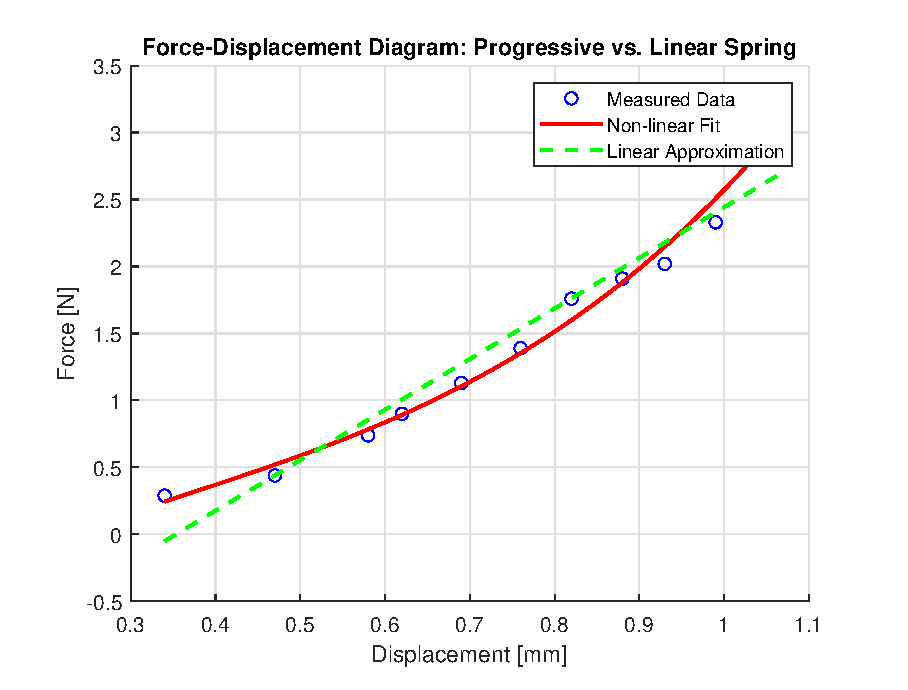
\includegraphics[width=0.62\textwidth]{img/SpringTest.eps}
    \caption[SpringTest]{SpringTest}
    \label{fig:SpringTest}
\end{figure}


\section{Limitations and Identified Challenges}

    \chapter[Formatierungen]{Formeln}\label{cha-formeln}

Ein besonderer Vorteil von \LaTeX ist die schnelle und einfache Art Formeln einzugeben. Mit ein wenig "Ubung in der Nomenklatur gehen die komplexesten Ausdr"ucke problemlos von der Hand. Eine einfache Formel sieht folgendermaßen.
\begin{equation}
p_1+\frac{\rho v_1^2}{2}+\rho gh_1=p_2+\frac{\rho v_2^2}{2}+\rho gh_2+\Delta p.
\label{eqn-bernoulli}
\end{equation}
Oft ziehen sich Formeln "uber mehrere Zeilen  
\begin{eqnarray}
\Delta L&=&\int\limits_0^L(1-\cos\varphi)\,dx\approx\int\limits_0^L[1-(1-\varphi^2/2)]\,dx=\frac{1}{2}\int\limits_0^Lw'^2\,dx=\nonumber\\
&=&\frac{B^2\lambda^2}{2}\int\limits_0^L\cos^2\lambda x\,dx=\frac{B^2\lambda^2}{2}\left[\frac{\lambda x-\sin\lambda x\cos\lambda x}{2\lambda}\right]_0^L\approx\frac{B^2\lambda^2L}{4}
\end{eqnarray}
oder sind sehr kompliziert
\begin{eqnarray}
\boldsymbol{\tau}&=&2\mu\mathbf{D}=\mu[\nabla\vec{v}+(\nabla\vec{v})^T]\\
\boldsymbol{\sigma}'&=&\mu'\nabla\cdot\,\vec{v}\,\mathbf{I}=-\frac{2}{3}\mu\,\nabla\cdot(\nabla{v})\,\mathbf{I}.
\end{eqnarray}


    \chapter{Evaluation}

    \chapter{Zusammenfassung und Ausblick}

    \chapter{Introduction}
\label{chapter:introduction}
\section{Sample text}
\label{section:sample_text}
\lipsum[1]
\section{Another sample text}
\label{section:another_sample_text}
\lipsum[2]
\chapter{Theoretical background}
\label{chapter:theoretical_bg}
\section{Some facts}
\label{section:some_facts}
\lipsum[1]
\section{Some more facts}
\label{section:some_more_facts}
\lipsum[2]
\chapter{Tips and Tricks}
\label{chapter:tips_and_tricks}
\section{Cross-referencing and citing}
\label{section:cross_ref_and_citing}

\begin{itemize}
	\item \num{1234,56}  % Zahl mit Dezimaltrennzeichen
	\item \SI{2}{\meter^{-1}} % Einheit m^-1 ohne Bruch
	\item \SI{1.23e4}{\newton\meter} % Exponenten mit Punkt als Produkt
	\item \SI{1000}{\kilo\ohm} % Tausender ohne Trennzeichen
\end{itemize}
\section{Circuits and graphs}
\label{section:circuits_and_graphs}
\Cref{fig:demo_circuit} shows a simple linear and time-independent circuit, which is created with the package \texttt{circuitikz}. When using the \texttt{tikzexternalize} feature, the \texttt{circuitikz} environment must be substituted with \texttt{tikzpicture}. 
\begin{figure}[htbp]
	\centering
	\begin{tikzpicture}[scale=1,transform shape,european inductors,european resistors,
    american voltages]
    % grid definition
    % \draw[step=0.5,black!20,thin] (-4,-2.5) grid (4,2.5);
    % circuit definition
    \draw (0,0) coordinate (A) to [R,l=$R_\mathrm{1}$] ++ (-3,0) coordinate (B);
    \draw (B) to [vsource,l=$V_\mathrm{1}$] ++ (0,-2) -- ++ (3,0) coordinate (C);
    \draw (C) to [R,l=$R_\mathrm{L}$] (A);
    \draw (A) to [R,l_=$R_\mathrm{2}$,*-] ++ (3,0) coordinate (D);
    \draw (D) to [vsource,l=$V_\mathrm{2}$] ++ (0,-2) to [short,-*] (C);
\end{tikzpicture}
% EOF
	\caption{A simple circuit}
	\label{fig:demo_circuit}
\end{figure}

Waveforms captured by an oscilloscope are depicte \cite{deutsch}, im Anhang ist dann ein weiterer
Code verknüpft siehe dazu \ref{lst:test_code} und in \cref{fig:demo_circuit} und \ref{fig:demo_circuit} ist ein Schaltkreis mit tikz gezeichnet.

    \pagenumbering{Roman} % use uppercase roman numerals for page numbering
	\setcounter{page}{\value{romanpagecount}} % set page number to the stored value
    \stepcounter{page} % increment the page counter
    \bibliography{IEEEabrv,mybibfile} % point BibTEX at the .bib files
	\addcontentsline{toc}{chapter}{\bibname}
    \clearpage
	\listoffigures % generate a list of all the figures
	\addcontentsline{toc}{chapter}{\listfigurename}
    \clearpage
	\listoftables % generate a list of all the tables
	\addcontentsline{toc}{chapter}{\listtablename}
	\clearpage
    \printglossary[type=acronym, title={Abkürzungsverzeichnis}] % input files created by MakeIndex
	\printglossary[type=symbolslist,style=symbolsliststyle, title={Symbolverzeichnis}]
    \appendix
    \chapter[Erster Anhang]{Überschrift des ersten Anhangs}\label{app-A}

\lstinputlisting[caption={Test}, label={lst:test_code}]{code/matlab_example.m}


\end{document}
%%%%%%%%%%%%%%%%%%%%%%%%%%%%%%%%%%%%%%%%%%%%%%%%%%%%%%%%%%%%%%%%%%%%%%%%%%%%%%%%%%%%%%